
\begin{figure}[ht]
    \centering
    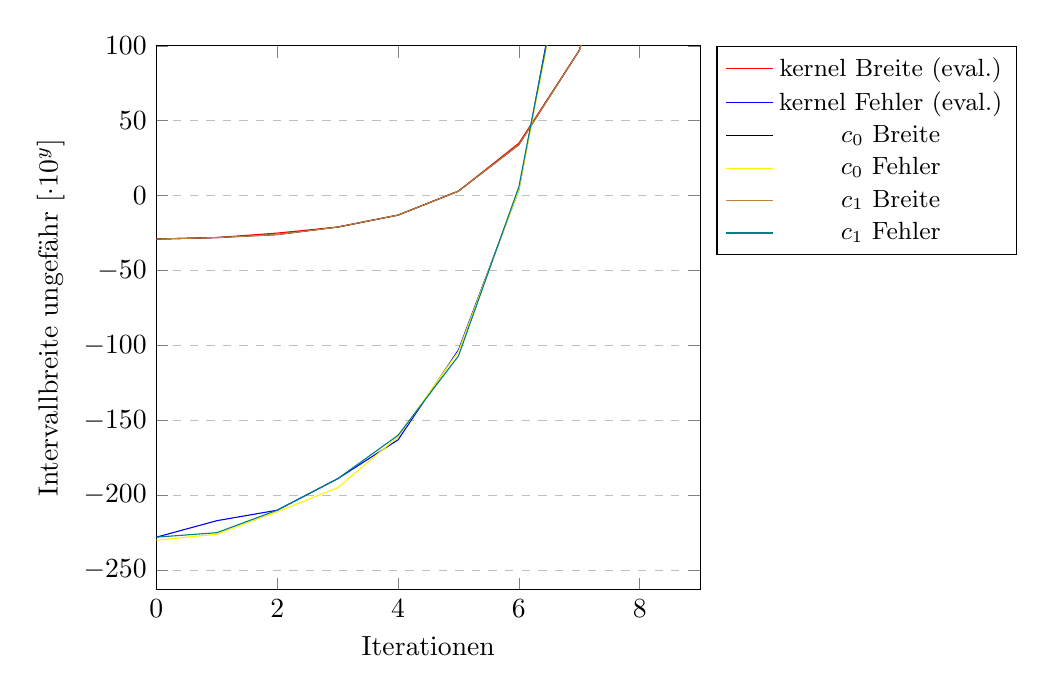
\begin{tikzpicture}
    \begin{axis}[
        width=0.7\textwidth,
        height=0.7\textwidth,
        xlabel={Iterationen},
        ylabel={Intervallbreite ungefähr $[\cdot 10^y ]$},
        legend pos=north west,
        xmin=0,xmax=9,
        ymax=100,
        ymajorgrids=true,
        grid style=dashed,
        legend pos=outer north east,
        cycle list name=color list
    ]
    
    \addplot
        coordinates {
 (0,-29)
 (1,-28)
 (2,-25)
 (3,-21)
 (4,-13)
 (5,03)
 (6,035)
 (7,097)
 (8,0223)
        };
        \addlegendentry{\small{kernel Breite (eval.)}}
    
    \addplot
        coordinates {
  (0,-228)
 (1,-217)
 (2,-210)
 (3,-189)
 (4,-163)
 (5,-103)
 (6,4)
 (7,220)
        };
        \addlegendentry{\small{kernel Fehler (eval.)}}
       
    
    \addplot
        coordinates {
 (0,-29)
 (1,-28)
 (2,-26)
 (3,-21)
 (4,-13)
 (5,03)
 (6,034)
 (7,097)
 (8,0223)
        };
        \addlegendentry{\small{$c_0$ Breite}}
        
    \addplot
        coordinates {
  (0,-230)
 (1,-226)
 (2,-211)
 (3,-195)
 (4,-161)
 (5,-104)
 (6,4)
 (7,212)
 (8,631)
        };
        \addlegendentry{\small{$c_0$ Fehler}}
    
        \addplot
        coordinates {
 (0,-29)
 (1,-28)
 (2,-26)
 (3,-21)
 (4,-13)
 (5,03)
 (6,034)
 (7,097)
 (8,0223)
        };
        \addlegendentry{\small{$c_1$ Breite}}
    
        \addplot
        coordinates {
   (0,-228)
 (1,-225)
 (2,-210)
 (3,-189)
 (4,-160)
 (5,-107)
 (6,6)
 (7,214)
        };
        \addlegendentry{\small{$c_1$ Fehler}}
    
    
    \end{axis}
    \end{tikzpicture}
    \caption{$x_0 = [0 \pm 0] + [0.5 \pm \varepsilon] \cdot \lambda,\  \lambda \in [1 \pm 0]$}
    \label{fig:tm4}
\end{figure}